\documentclass{article}

% Language setting
% Replace `english' with e.g. `spanish' to change the document language
\usepackage[english]{babel}
\usepackage{booktabs}
\usepackage{float}
\usepackage{caption}
\usepackage{tikz}
\usetikzlibrary{positioning,arrows.meta,fit,backgrounds,calc}
\usepackage{graphicx} % only needed for \resizebox


% Set page size and margins
% Replace `letterpaper' with `a4paper' for UK/EU standard size
\usepackage[letterpaper,top=2cm,bottom=2cm,left=3cm,right=3cm,marginparwidth=1.75cm]{geometry}

% Useful packages
\usepackage{amsmath}
\usepackage{graphicx}
\usepackage[colorlinks=true, allcolors=blue]{hyperref}

\title{Dial-Up: Networking Over Sound}
\author{Jagger Winkler, Arthur Ufongene}
\date{\today}

\begin{document}

\maketitle

\section{Introduction}
The goal of this project is to design and implement a networking protocol that can transmit data over sound. 
This project implements layers one and two of the OSI model, the physical layer and the data link layer. 
The physical layer is responsible for transmitting raw bits over a communication channel, 
while the data link layer is responsible for providing reliable data transfer between two devices on the same network.

\section{Pipeline}

The project is split into two layers, the physical layer and the data link layer. The data link layer is Responsible for framing, addressing, and detecting corrupted frames,
similar to its role in the Ethernet protocol. The physical layer is responsibe for modulating the data into sound and demodulating the sound back into data, alongside
a large amount of error correction.

\begin{figure}[htbp]
\centering
\resizebox{\linewidth}{!}{%
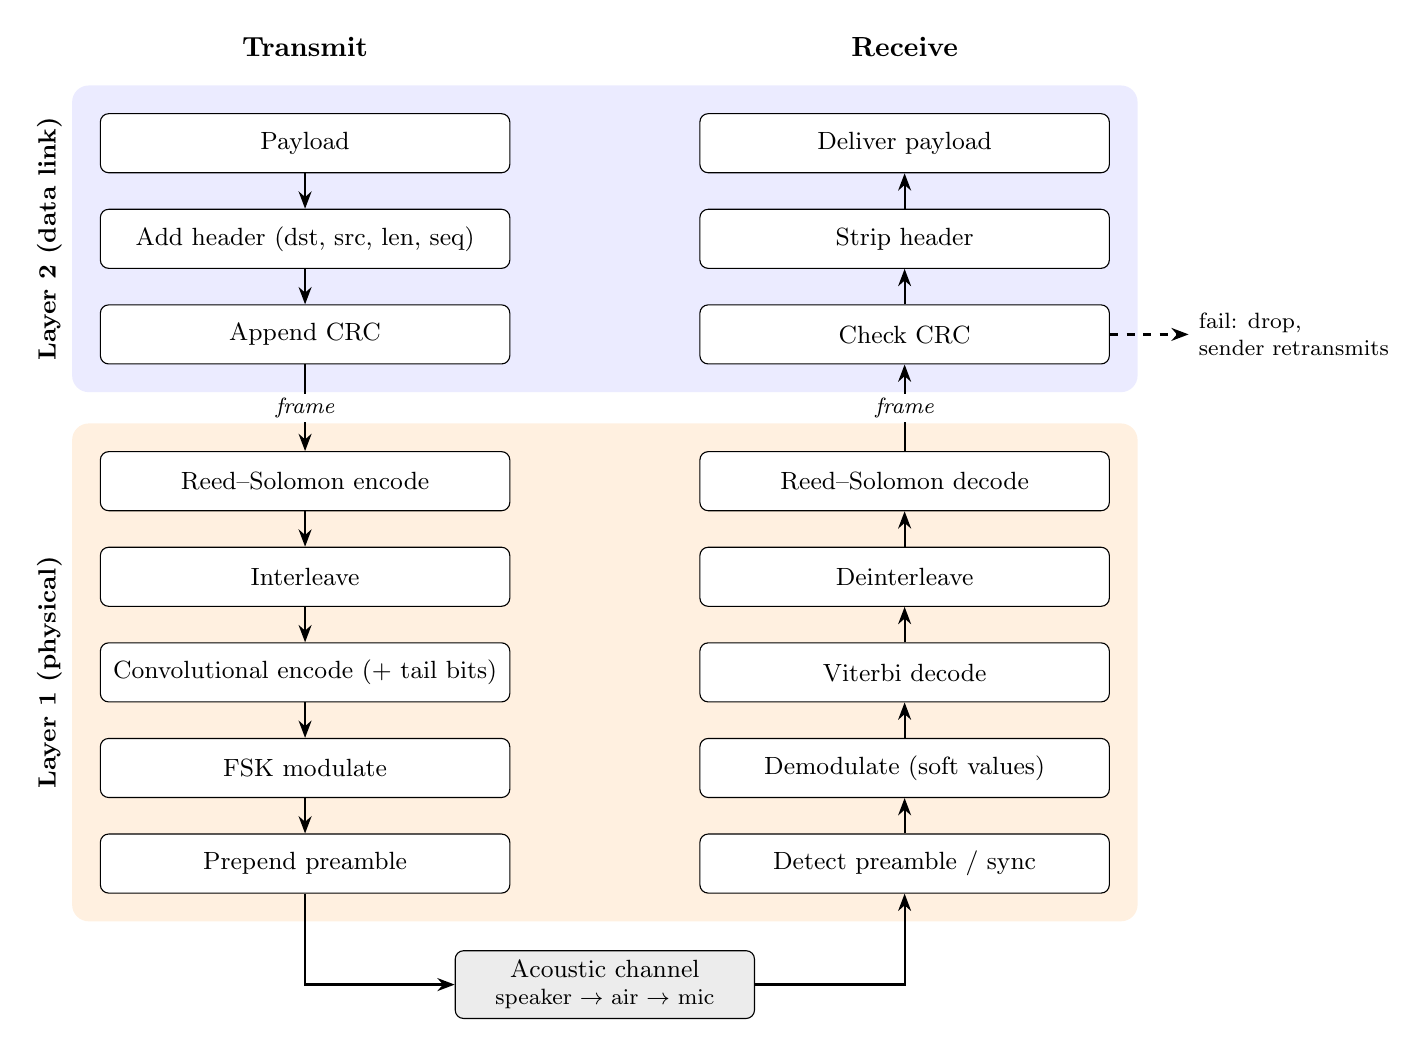
\begin{tikzpicture}[
  node distance=0.45cm,
  block/.style={draw, rounded corners=3pt, minimum width=5.2cm,
                minimum height=0.75cm, font=\small, fill=white, align=center},
  arr/.style={-{Stealth[length=2.2mm]}, thick},
  layer/.style={rounded corners=6pt, inner sep=10pt},
  lbl/.style={font=\footnotesize\itshape, fill=white, inner sep=1.5pt},
]
 
% ---------------- Transmit (top to bottom) ----------------
\node[block] (t1) {Payload};
\node[block, below=of t1] (t2) {Add header (dst, src, len, seq)};
\node[block, below=of t2] (t3) {Append CRC};
\node[block, below=1.1cm of t3] (t4) {Reed--Solomon encode};
\node[block, below=of t4] (t5) {Interleave};
\node[block, below=of t5] (t6) {Convolutional encode (+ tail bits)};
\node[block, below=of t6] (t7) {FSK modulate};
\node[block, below=of t7] (t8) {Prepend preamble};
 
% ---------------- Receive (bottom to top) -----------------
\node[block, right=2.4cm of t1] (r1) {Deliver payload};
\node[block, below=of r1] (r2) {Strip header};
\node[block, below=of r2] (r3) {Check CRC};
\node[block, below=1.1cm of r3] (r4) {Reed--Solomon decode};
\node[block, below=of r4] (r5) {Deinterleave};
\node[block, below=of r5] (r6) {Viterbi decode};
\node[block, below=of r6] (r7) {Demodulate (soft values)};
\node[block, below=of r7] (r8) {Detect preamble / sync};
 
% ---------------- Channel ----------------
\node[block, minimum width=3.8cm, fill=gray!15,
      below=1.1cm of $(t8)!0.5!(r8)$] (ch)
      {Acoustic channel\\[-1pt]{\footnotesize speaker $\rightarrow$ air $\rightarrow$ mic}};
 
% ---------------- Arrows ----------------
\foreach \a/\b in {t1/t2, t2/t3, t3/t4, t4/t5, t5/t6, t6/t7, t7/t8}
  \draw[arr] (\a) -- (\b);
\foreach \a/\b in {r8/r7, r7/r6, r6/r5, r5/r4, r4/r3, r3/r2, r2/r1}
  \draw[arr] (\a) -- (\b);
 
\draw[arr] (t8.south) |- (ch.west);
\draw[arr] (ch.east) -| (r8.south);
 
\path (t3) -- (t4) node[midway, lbl] {frame};
\path (r4) -- (r3) node[midway, lbl] {frame};
 
% CRC failure branch
\draw[arr, dashed] (r3.east) -- ++(1.0,0)
  node[right, font=\footnotesize, align=left] {fail: drop,\\sender retransmits};
 
% ---------------- Column headers ----------------
\node[font=\bfseries, above=0.6cm of t1] {Transmit};
\node[font=\bfseries, above=0.6cm of r1] {Receive};
 
% ---------------- Layer bands ----------------
\begin{scope}[on background layer]
  \node[layer, fill=blue!8,   fit=(t1)(r3)] (L2) {};
  \node[layer, fill=orange!12, fit=(t4)(r8)] (L1) {};
\end{scope}
\node[rotate=90, anchor=south, font=\bfseries\small] at (L2.west)
  {Layer 2 (data link)};
\node[rotate=90, anchor=south, font=\bfseries\small] at (L1.west)
  {Layer 1 (physical)};
 
\end{tikzpicture}
}% end resizebox
\caption{Acoustic link pipeline}
\label{fig:acoustic-pipeline}
\end{figure}

\subsection{Layer 2 Transmit}

\subsection{Layer 1 Transmit}

\subsection{Layer 1 Receive}

\subsection{Layer 2 Receive}

\section{Acknowledgements}
Figures were generated with the help of Claude Opus 5.5, by describing every component of the figure in detail. The figure was then refined and polished by the authors.
\end{document}